

\tikzset{every picture/.style={line width=0.75pt}} %set default line width to 0.75pt        

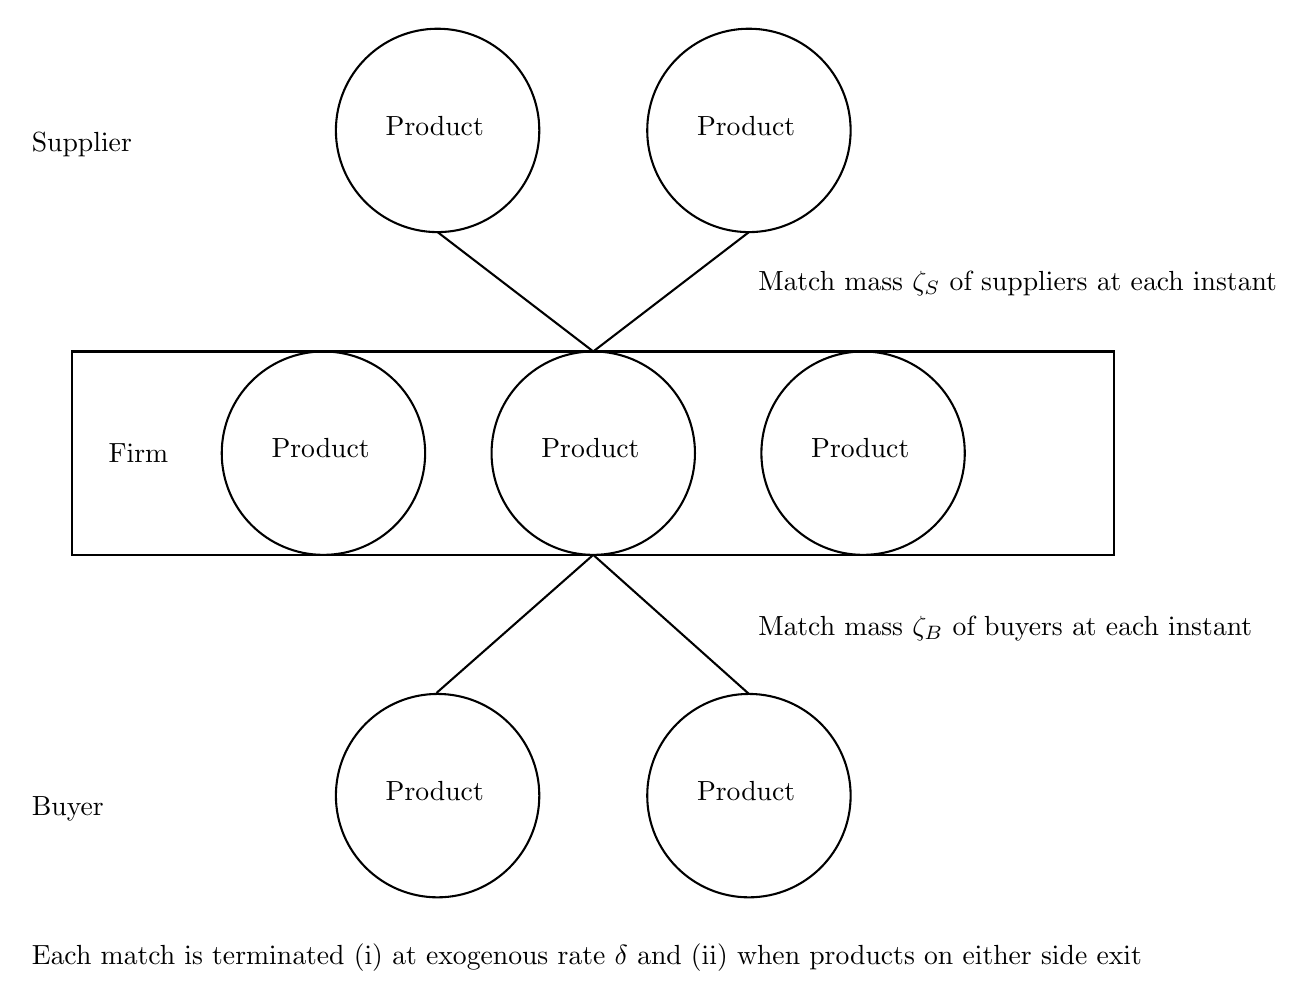
\begin{tikzpicture}[x=0.75pt,y=0.75pt,yscale=-1,xscale=1]
  %uncomment if require: \path (0,501); %set diagram left start at 0, and has height of 501

  %Shape: Circle [id:dp49239278227487526] 
  \draw   (275,219) .. controls (275,191.94) and (296.94,170) .. (324,170) .. controls (351.06,170) and (373,191.94) .. (373,219) .. controls (373,246.06) and (351.06,268) .. (324,268) .. controls (296.94,268) and (275,246.06) .. (275,219) -- cycle ;
  %Shape: Rectangle [id:dp3686127216176238] 
  \draw   (73,170) -- (575,170) -- (575,268) -- (73,268) -- cycle ;
  %Shape: Circle [id:dp44429653969502425] 
  \draw   (145,219) .. controls (145,191.94) and (166.94,170) .. (194,170) .. controls (221.06,170) and (243,191.94) .. (243,219) .. controls (243,246.06) and (221.06,268) .. (194,268) .. controls (166.94,268) and (145,246.06) .. (145,219) -- cycle ;
  %Shape: Circle [id:dp2627879599683287] 
  \draw   (405,219) .. controls (405,191.94) and (426.94,170) .. (454,170) .. controls (481.06,170) and (503,191.94) .. (503,219) .. controls (503,246.06) and (481.06,268) .. (454,268) .. controls (426.94,268) and (405,246.06) .. (405,219) -- cycle ;
  %Shape: Circle [id:dp7882477687030796] 
  \draw   (200,63.5) .. controls (200,36.44) and (221.94,14.5) .. (249,14.5) .. controls (276.06,14.5) and (298,36.44) .. (298,63.5) .. controls (298,90.56) and (276.06,112.5) .. (249,112.5) .. controls (221.94,112.5) and (200,90.56) .. (200,63.5) -- cycle ;
  %Shape: Circle [id:dp22656680762974557] 
  \draw   (350,63.5) .. controls (350,36.44) and (371.94,14.5) .. (399,14.5) .. controls (426.06,14.5) and (448,36.44) .. (448,63.5) .. controls (448,90.56) and (426.06,112.5) .. (399,112.5) .. controls (371.94,112.5) and (350,90.56) .. (350,63.5) -- cycle ;
  %Shape: Circle [id:dp1646559994356671] 
  \draw   (200,384) .. controls (200,356.94) and (221.94,335) .. (249,335) .. controls (276.06,335) and (298,356.94) .. (298,384) .. controls (298,411.06) and (276.06,433) .. (249,433) .. controls (221.94,433) and (200,411.06) .. (200,384) -- cycle ;
  %Shape: Circle [id:dp782733553592635] 
  \draw   (350,384) .. controls (350,356.94) and (371.94,335) .. (399,335) .. controls (426.06,335) and (448,356.94) .. (448,384) .. controls (448,411.06) and (426.06,433) .. (399,433) .. controls (371.94,433) and (350,411.06) .. (350,384) -- cycle ;
  %Straight Lines [id:da5188898566840481] 
  \draw    (249,112.5) -- (324,170) ;
  %Straight Lines [id:da48490872000378227] 
  \draw    (399,112.5) -- (324,170) ;
  %Straight Lines [id:da042544601454206576] 
  \draw    (324,268) -- (248.5,334.5) ;
  %Straight Lines [id:da14755230855670742] 
  \draw    (324,268) -- (399,335) ;

  % Text Node
  \draw (297.5,210.5) node [anchor=north west][inner sep=0.75pt]   [align=left] {Product};
  % Text Node
  \draw (89,213) node [anchor=north west][inner sep=0.75pt]   [align=left] {Firm};
  % Text Node
  \draw (167.5,210.5) node [anchor=north west][inner sep=0.75pt]   [align=left] {Product};
  % Text Node
  \draw (427.5,210.5) node [anchor=north west][inner sep=0.75pt]   [align=left] {Product};
  % Text Node
  \draw (222.5,55) node [anchor=north west][inner sep=0.75pt]   [align=left] {Product};
  % Text Node
  \draw (372.5,55) node [anchor=north west][inner sep=0.75pt]   [align=left] {Product};
  % Text Node
  \draw (222.5,375.5) node [anchor=north west][inner sep=0.75pt]   [align=left] {Product};
  % Text Node
  \draw (372.5,375.5) node [anchor=north west][inner sep=0.75pt]   [align=left] {Product};
  % Text Node
  \draw (52,63) node [anchor=north west][inner sep=0.75pt]   [align=left] {Supplier};
  % Text Node
  \draw (52,383) node [anchor=north west][inner sep=0.75pt]   [align=left] {Buyer};
  % Text Node
  \draw (402,130) node [anchor=north west][inner sep=0.75pt]   [align=left] {Match mass $\displaystyle \zeta _{S}$ of suppliers at each instant};
  % Text Node
  \draw (402,296) node [anchor=north west][inner sep=0.75pt]   [align=left] {Match mass $\displaystyle \zeta _{B}$ of buyers at each instant};
  % Text Node
  \draw (52,454) node [anchor=north west][inner sep=0.75pt]   [align=left] {Each match is terminated (i) at exogenous rate $\displaystyle \delta $ and (ii) when products on either side exit };


\end{tikzpicture}


